\documentclass{article}

% For many columns
\usepackage{multicol}
% For vertical brace rcases
\usepackage{mathtools}
% For positioning figures
\usepackage{float}
% makes figure font bold
\usepackage{caption}
\captionsetup[figure]{labelfont=bf}
% For text generation
\usepackage{lipsum}
% For drawing
\usepackage{tikz}
\usepackage{tikz-3dplot}
% For manipulating coordinates
\usetikzlibrary{calc}
% For smaller or equal sign and not divide sign
\usepackage{amssymb}
% For the diagonal fraction
\usepackage{xfrac}
% For enumerating exercise parts with letters instead of numbers
\usepackage{enumitem}
% For dfrac, which forces the fraction to be in display mode (large) e
% even in math mode (small)
\usepackage{amsmath}
% For degree sign
\usepackage{gensymb}
% For "\mathbb" macro
\usepackage{amsfonts}
\newcommand{\N}{\mathbb{N}}
\newcommand{\Z}{\mathbb{Z}}
\newcommand{\Q}{\mathbb{Q}}
\newcommand{\R}{\mathbb{R}}
\newcommand{\C}{\mathbb{C}}
\newcommand{\F}{\mathbb{F}}
\newcommand{\rad}{\text{ rad}}
\newcommand{\orbit}{\mathcal{O}}
\newcommand{\Ccal}{\mathcal{C}}
\newcommand{\Pcal}{\mathcal{P}}
\newcommand{\Scal}{\mathcal{S}}

% overline short italic
\newcommand{\olsi}[1]{\,\overline{\!{#1}}}

\title{%
    \Huge Abstract Algebra \\
    \large by \\
    \Large Dummit and Foote \\~\\
    \huge Part 1: Group Theory \\
    \LARGE Chapter 1: Introduction to Groups \\
    \Large Section 7: Group Actions
}
\date{2023-07-14}
\author{Michael Saba}

\begin{document}
    \pagenumbering{gobble}
    \maketitle
    \newpage
    \pagenumbering{arabic}


    \section*{Exercise 1}
    Proof that in a field $F$, the multiplicative group
    $F^\times = F - \{0\}$ (where 0 is the addi identity),
    acts on the set $F$ with $g \cdot a = ga$ for $\forall g \in F^\times$
    and $\forall a \in F$: \\
    For $g_1, g_2 \in F^\times$ and $a \in F$,
    since multiplication is asosciative in fields,
    we have $g_1 \cdot (g_2 \cdot a) = (g_1g_2) \cdot a$.
    Moreover, for the identity 1 of $F^\times$,
    $\forall a \in F$, we have $1 \cdot a = a$.
    So it is a group action.


    \section*{Exercise 2}
    Proof that $(\Z, +)$ acts on itself by $z \cdot a = z + a$
    $\forall z, a \in \Z$: \\
    In $\Z$, 0 is the identity, and $0 \cdot a = 0 + a = a$,
    while $\forall a, b \in \Z$,
    $a \cdot (b \cdot z) = a + (b + z) = (a + b) + z = (a + b) \cdot z$.
    So it is a group action.


    \section*{Exercise 3}
    Proof that $(\R, +)$ acts on $\R^2$
    where for $r, x, y \in \R$, $r \cdot (x, y) = (x + ry, y)$: \\
    For $r, s \in \R$,
    $r \cdot (s \cdot (x, y)) = r \cdot (x + sy, y)
    = (x + ry + sy, y)
    = (x + (r + s)y, y)
    = (r + s) \cdot (x, y)$
    And $0 \cdot (x, y) = (x + 0 \cdot y, y) = (x, y)$.
    So it is a group action.


    \section*{Exercise 4 $***$}
    Consider a group $G$ that acts on a set $A$
    and fix an element $a \in A$. \\
    \begin{enumerate}[label=\textbf{\alph*.}]
        \item 
            Proof that the kernel of the action is a subgroup of $G$.
            (The group action kernel is the set of elements in $G$ that
            map all elements of $A$ to themselves): \\
            Using two different approaches: \\
            We know that the kernel is the set of elements $g \in G$
            such that $\forall a \in A$, $g \cdot a = a$.
            We also know that the kernel of a homomorphism is the set
            of elements that the homomorphism maps to the identity of
            the second group. \\ 
            Moreover, we know that the group action corresponds to
            a homomorphism $\phi: G \to S_A$
            called a \textit{permutation representation},
            and defined by $\phi(g) = \sigma$
            such that $\forall a \in A$, $\sigma(a) = g \cdot a$
            (since the group action permutes the elments of the set
            it acts on). \\
            The kernel of $\phi$ is thus the set of elements that
            $\phi$ maps to the identity of $S_A$, corresponding
            to the elements of $G$ that don't permute any of $A$'s elements,
            but map each element to itself.
            So the kernel of the group action is the same as the kernel
            of the permutation representation homomorphism. \\
            We already showed in exercise 1.1.6.14 that the kernel
            of any homomorphism $\varphi: G \to H$ is a subgroup of $G$,
            so we conclude that the kernel of the group action is
            a subrgoup of $G$. \\
            Alternatively, we can use the new definition of the group action
            kernel to prove it's a subgroup of $G$: \\
            We know by the definition of the action that 1 belongs
            in the kernel as $1 \cdot a = a$ $\forall a \in A$.
            We also know, again by the associativity of the action that
            the kernel is closed under the group operation
            as $(g_1g_2) \cdot a = g_1 \cdot (g_2 \cdot a) = g_1 \cdot a = a$, 
            so $g_1g_2$ belongs in the kernel
            $\forall g_1, g_2$ also in the kernel.
            And we know that the inverse of $g$ in $G$, $g^{-1}$,
            is in the kernel since $1 \cdot a = a$,
            which means that $g^{-1}g \cdot a = 1$,
            hence $g^{-1} \cdot (g \cdot a) = 1$,
            which implies that $g^{-1} \cdot a = 1$.
            So the kernel is closed under inverses and the group operation,
            and is a non-empty subset of $G$,
            making it a subgroup.
        \item
            Proof that the \textit{stabilizer of $a$ in $G$},
            which is the set $G_a = \{ g \in G \mid g \cdot a = a \}$
            for a fixed $a$,
            is a subgroup of $G$: \\
            We know by the definition of the action that 1 belongs
            in $G_a$ as $1 \cdot a = a$ (which applies to all elements in $A$).
            We also know, again by the associativity of the action that
            the kernel is closed under the group operation
            as $(g_1g_2) \cdot a = g_1 \cdot (g_2 \cdot a) = g_1 \cdot a = a$, 
            so $g_1g_2$ belongs in the kernel $\forall g_1, g_2 \in G_a$.
            And we know that the inverse of $g$ in $G$, $g^{-1}$,
            is in the stablizier of $a$ since $1 \cdot a = a$,
            which means that $g^{-1}g \cdot a = 1$,
            hence $g^{-1} \cdot (g \cdot a) = 1$,
            which implies that $g^{-1} \cdot a = 1$.
            So $G_a$ is closed under inverses and the group operation,
            and is a non-empty subset of $G$,
            so $G_a \leqslant G$.
    \end{enumerate}


    \section*{Exercise 5}
    As we showed in exercise 1.1.7.4,
    we know that the kernel of an action is the set of elements $g \in G$
    such that $\forall a \in A$, $g \cdot a = a$.
    We also know that the kernel of a homomorphism is the set of elements
    that the homomorphism maps to the identity of the second group. \\ 
    Moreover, we know that the group action corresponds to a
    homomorphism $\phi: G \to S_A$
    called a \textit{permutation representation},
    and defined by $\phi(g) = \sigma$
    such that $\forall a \in A$, $\sigma(a) = g \cdot a$
    (since the group action permutes the elments of the set it acts on). \\
    The kernel of $\phi$ is thus the set of elements that
    $\phi$ maps to the identity of $S_A$, corresponding
    to the elements of $G$ that don't permute any of $A$'s elements,
    but map each element to itself.
    So the kernel of the group action is the same as the kernel of
    the permutation representation homomorphism. \\

    \section*{Exercise 6 $***$}
    Proof that a group $G$ acts faithfully on a set $A$ if and only
    if the kernel of the action contains only the identity of $G$
    (A group acts \textit{faithfully} on a set
    if no two elements in the group permute the set in the same way
    in other words, if the homomorphism of the permutation representation
    is injective, with each element mapping to a different permutation): \\
    First we assume that the kernel of the action $k =\{1\}$.
    Now let us assume that the action does not act faithfully on $A$,
    meaning that $\exists g_1, g_2 \in G$
    such that $g_1 \neq g_2$, $g_1, g_2 \neq 1$,
    and $g_1 \cdot a = g_2 \cdot a$ for all values $a \in A$.
    We know that
    $g_1^{-1} \cdot g_1 \cdot a = (g_1^{-1}g_1) \cdot a = 1 \cdot a = a$,
    so $g_1^{-1} \cdot g_2 \cdot a$,
    which implies that $\forall a \in A$,
    $(g_1^{-1}g_2) \dot a = a$.
    This tells us that $g_1^{-1}g_2$ is in the kernel,
    but $g_1^{-1}g_2 \neq 1$
    since we assumed that $g_1 \neq g_2$ and $g_1, g_2 \neq 1$.
    This is contradiction of our assumption that $k =\{1\}$,
    so we conclude that the action must be faithful. \\
    Conversely, if we assume the action is faithful,
    then we know that no two elements in $G$ permute $A$ identically.
    We also know that $1 \dot a = a$ $\forall a \in A$.
    No element beside 1 can have this exact mapping,
    so no element but 1 can be part of the kernel.
    So $k = \{1\}$.


    \section*{Exercise 7}
    Consider the action of the group $F^\times$ on a vector space $V$
    over the field $F$ defined by $\alpha \cdot (r_1, r_2, \dots r_n)
    = (\alpha \cdot r_1, \alpha \cdot r_2, \dots \alpha \cdot r_n)$
    $\forall \alpha \in F^\times$ and $r_i \in F$.
    (the action of $\alpha$ on each individual $r_i$ is the one that
    was proved to be an action in exercise 1.1.7.1).
    Proof that this action is faithful when $F = \R$ and $V = \R^n$: \\
    We know that for the multiplicative identity 1 of $F^\times$,
    \[ 1 \cdot (r_1, r_2, \dots r_n) =
    (1 \cdot r_1, 1 \cdot r_2, \dots 1 \cdot r_n)
    = (r_1, r_2, \dots r_n) \]
    Moreover, $\forall \alpha, \beta \in F^\times$,
    \[ \alpha \cdot \beta \cdot (r_1, r_2, \dots r_n)
    = \beta \cdot (\beta r_1, \beta r_2, \dots \beta r_n)
    = (\alpha (\beta r_1), \alpha (\beta r_2),
    \dots \alpha (\beta r_n)) \]
    and because multiplication is associative in $\R$, this is equal to
    \[((\alpha \beta) r_1, (\alpha \beta) r_2,
    \dots (\alpha \beta) r_n)
     = (\alpha \beta) \cdot (r_1, r_2, \dots r_n) \]
    which makes this a group action.
    (Note that this result is true for any field,
    since the group action of $F^\times$ on $V$ only requires that
    $F^\times$ act on $F$, the tuples in a vector space,
    which we proved was the case in exercise 1.1.7.1). \\
    Now to show that the action is faithful,
    we assume that there exists two elements $\alpha, \beta \in F^\times$
    such that $\forall v \in V$, $\alpha \cdot v = \beta \cdot v$.
    This implies that $\forall r_i \in v$,
    $\alpha r_i = \beta r_i$.
    Since $r_i \in \R$,
    we have $\alpha r_i - \beta r_i = 0$.
    So $(\alpha - \beta) r_i = 0$,
    which means that $(\alpha - \beta) = 0$,
    so $\alpha = \beta$.
    So we may conclude that the action must be faithful.


    \section*{Exercise 8}
    Let $A$ be a non-empty set and $k$ be a positive integer
    such that $k \leqslant |A|$.
    Now consider the group $S_A$ which acts on the set $B$
    which consists of all subsests of $A$ with cardinality $k$
    by $\sigma \cdot \{a_1, a_2 \dots a_k\} =
    \{\sigma(a_1), \sigma(a_2) \dots \sigma(a_k)\}$. \\
    \begin{enumerate}[label=\textbf{\alph*.}]
        \item 
            Proof that this is a group action: \\
            We have 
            \[ 1 \cdot \{a_1, a_2 \dots a_k\}
            = \{1(a_1), 1(a_2) \dots 1(a_k)\}
            = \{a_1, a_2 \dots a_k\} \]
            And for any permutations $\sigma, \pi \in S_A$
            \[ \sigma \cdot \pi \cdot \{a_1, a_2 \dots a_k\}
            = \sigma \cdot \{\pi(a_1), \pi(a_2) \dots \pi(a_k)\} \]
            \[ = \{\sigma(\pi(a_1)), \sigma(\pi(a_2))
            \dots \sigma(\pi(a_k))\} \]
            which is equal to
            \[ \{(\sigma \circ \pi)(a_1), (\sigma \circ \pi)(a_2)
            \dots (\sigma \circ \pi)(a_n)\}
            = (\sigma \circ \pi)(\{a_1, a_2 \dots a_k\}) \] 
            since composition is associative in $S_A$. 
            We conclude that it is a group action.
        \item 
            For $k = 2$ and $A \{1, 2, 3, 4\}$,
            we have
            \[B = \{\{1, 2\}, \{1, 3\}, \{1, 4\}, \{2, 3\}, \{2, 4\},
            \{3, 4\}\}\]
            \begin{multicols}{2}
                For $\sigma = (1\;2)$, we have: \\
                $\sigma(\{1, 2\}) = \{1, 2\} \\
                \sigma(\{1, 3\}) = \{2, 3\} \\
                \sigma(\{1, 4\}) = \{2, 4\} \\
                \sigma(\{2, 3\}) = \{1, 3\} \\
                \sigma(\{2, 4\}) = \{1, 4\} \\
                \sigma(\{3, 4\}) = \{3, 4\}$ \\
                % No idea why I need to add the line break
                \columnbreak \\
                And for $\sigma = (1\;2\;3)$ we have: \\
                $\sigma(\{1, 2\}) = \{2, 3\} \\
                \sigma(\{1, 3\}) = \{1, 2\} \\
                \sigma(\{1, 4\}) = \{2, 4\} \\
                \sigma(\{2, 3\}) = \{1, 3\} \\
                \sigma(\{2, 4\}) = \{3, 4\} \\
                \sigma(\{3, 4\}) = \{1, 4\}$ \\
            \end{multicols}
    \end{enumerate}


    \section*{Exercise 9}
    Let $A$ be a non-empty set and $k$ be a positive integer
    such that $k \leqslant |A|$.
    Now consider the group $S_A$ which acts on the set $B$
    which consists of all ordered $k$-tuples containing elements of $A$
    by $\sigma \cdot (a_1, a_2 \dots a_k) =
    (\sigma(a_1), \sigma(a_2) \dots \sigma(a_k))$. \\
    \begin{enumerate}[label=\textbf{\alph*.}]
        \item 
            Proof that this is a group action: \\
            We have 
            \[ 1 \cdot (a_1, a_2 \dots a_k)
            = (1(a_1), 1(a_2) \dots 1(a_k))
            = (a_1, a_2 \dots a_k) \]
            And for any permutations $\sigma, \pi \in S_A$
            \[ \sigma \cdot \pi \cdot (a_1, a_2 \dots a_k)
            = \sigma \cdot \{\pi(a_1), \pi(a_2) \dots \pi(a_k)\} \]
            \[ = (\sigma(\pi(a_1)), \sigma(\pi(a_2))
            \dots \sigma(\pi(a_k))) \]
            which is equal to
            \[ ((\sigma \circ \pi)(a_1), (\sigma \circ \pi)(a_2)
            \dots (\sigma \circ \pi)(a_n))
            = (\sigma \circ \pi)((a_1, a_2 \dots a_k)) \] 
            since composition is associative in $S_A$. 
            We conclude that it is a group action.
        \item 
            For $k = 2$ and $A \{1, 2, 3, 4\}$,
            we have
            \[ B = \{(1, 2), (1, 3), (1, 4), (2, 3), (2, 4),
            (3, 4), (2, 1), (3, 1), (4, 1), (3, 2), \]
            \[ (4, 2),(4, 3)\} \]
            \begin{multicols}{2}
                For $\sigma = (1\;2)$, we have: \\
                $\sigma((1, 2)) = (2, 1) \\
                \sigma((1, 3)) = (2, 3) \\
                \sigma((1, 4)) = (2, 4) \\
                \sigma((2, 3)) = (1, 3) \\
                \sigma((2, 4)) = (1, 4) \\
                \sigma((3, 4)) = (3, 4) \\
                \sigma((2, 1)) = (1, 2) \\
                \sigma((3, 1)) = (3, 2) \\
                \sigma((4, 1)) = (4, 2) \\
                \sigma((3, 2)) = (3, 1) \\
                \sigma((4, 2)) = (4, 1) \\
                \sigma((4, 3)) = (4, 3)$ \\
                % No idea why I need to add the line break
                \columnbreak \\
                And for $\sigma = (1\;2\;3)$ we have: \\
                $\sigma((1, 2)) = (2, 1) \\
                \sigma((1, 3)) = (2, 1) \\
                \sigma((1, 4)) = (2, 4) \\
                \sigma((2, 3)) = (3, 1) \\
                \sigma((2, 4)) = (3, 4) \\
                \sigma((3, 4)) = (1, 4) \\
                \sigma((2, 1)) = (1, 2) \\
                \sigma((3, 1)) = (1, 2) \\
                \sigma((4, 1)) = (4, 2) \\
                \sigma((3, 2)) = (1, 3) \\
                \sigma((4, 2)) = (4, 3) \\
                \sigma((4, 3)) = (4, 1)$ \\
            \end{multicols}
    \end{enumerate}


    \section*{Exercise 10 $***$}
    With reference to exercises 1.1.7.8 and 1.1.7.9: \\
    \begin{enumerate}[label=\textbf{\alph*.}]
        \item 
            In exercise 1.1.7.8,
            where $B$ is the set of subsets of $A$ of size $k$,
            the action of $S_A$ on $B$ is faithful for all $k$,
            such that $1 \leqslant k < |A|$.
            To prove this: \\
            Assume that two permutations $\sigma, \pi \in S_A$
            are distinct permutations,
            meaning that $\exists a \in A$ such that $\sigma(a) \neq \pi(a)$.
            Then $a$ belongs to some subsets of $A$ in $B$.
            If $k = 1$, then for the subset ${a}$,
            $\sigma({a}) = {\sigma(a)} \neq {\pi(a)} = \pi({a})$,
            so there always exists an element in $B$ such that
            $\sigma$ and $\pi$ permute it differently. \\
            Otherwise, if $1 < k < |A|$,
            then consider a susbet of $A$ in $B$ that contains $a$
            and call it $S$.
            Although $a \in S$ and $\sigma(a) \neq \pi(a)$,
            it may still be possible that $\sigma \cdot S = \pi \cdot S$.
            This is because while $a$ maps to a different element
            in each case,
            the sets may still be equal since they are unordered
            and the mapping of other elements can make up for the difference.
            To show that there is at least such a subset containing $a$
            that won't be mapped the same way by both perumtations,
            take $b = \sigma(a)$.
            For the two sets $\sigma \cdot S$ and $\pi \cdot S$ to be equal,
            there must be an element $c \in S$ such that $\pi(c) = b$.
            This element is unique since $\pi$ is a permutation.
            Now, since we have $k < |A|$,
            there must be at least one subset $S$ of $A$
            that contains $a$ but not $c$.
            In such a case $\sigma \cdot S$ contains $b$,
            but $\pi \cdot S$ doesn't
            (again, because $c$ is the only element that maps to be,
            since $\pi$ is a permutation).
            So if $\sigma \neq \pi$ where $\sigma(a) \neq \sigma(b)$,
            then there will always be one $S \in B$ such that
            $\sigma \cdot S \neq \pi \cdot S$,
            where $S$ is the subset of $A$ containing $a$
            but not $\pi^{-1}(\sigma(a))$ (which we called c).
            If $k = |A|$ however, since $\pi$ and $\sigma$ are permutations,
            the one subset of $A$ in $B$ is $A$ itself,
            and permuting it gives the same set as $A$ is unordered.
            So no two distinct permutations act on $B$ in the same way
            for $1 \leqslant k < |A|$,
            which makes the action is faithful so long as $k \neq |A|$.
        \item
            In exercise 1.1.7.9,
            where $B$ is the set of $k$-tuples with elements in $A$,
            the action of $S_A$ on $B$ is faithful for all $k$,
            such that $1 \leqslant k \leqslant |A|$.
            To prove this: \\
            Assume that two permutations $\sigma, \pi \in S_A$
            are distinct permutations,
            meaning that $\exists a \in A$ such that $\sigma(a) \neq \pi(a)$.
            Then $a$ belongs to some $k$-tuple of $A$ in $B$.
            Let's call such a tuple $S$.
            In $S$, $\sigma \cdot S$ will map $a$ to a different element
            than $\pi \cdot S$ will.
            Since $S$ is ordered,
            that means that $\sigma \cdot S \neq \pi \cdot S$.
            Since for all distinct permutations, there will always exist
            such tuples,
            then we can conclude that the action on $B$ is faithful
            for all values of $k$.
    \end{enumerate}


    \section*{Exercise 11}
    Consider the action of $D_8$ on the set $S = {1, 2, 3, 4}$
    where $S$ represents the vertices of a square labeled clockwise
    and the action permutes the set in the same way each transformation
    in $D_8$ moves the vertices of the square.
    The group $D_8$ can be mapped to $S_4$ through its permutation
    representation homomorphism,
    where each transformation in $D_8$ maps to the permutation in $S_4$
    that permutes $S$ in the same way the transformation does. \\

    \begin{figure}[H]
        \centering
        % figure is a tikz drawing
        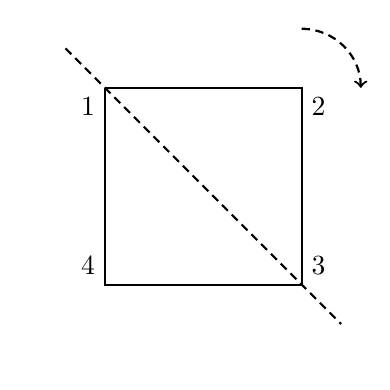
\begin{tikzpicture}[scale=2.5]
    
        \pgfmathsetmacro{\side}{1}

        % Specifies where the x, y coordinate of the tip of
        % the unite vectors in turn
        \tikzset{}
        
        % Scope used to shift the coordinates from the basis
        \begin{scope}[shift={(0, 0, 0)}, rotate=0]
            \coordinate (A1) at (0, \side);
            \coordinate (A2) at (\side, \side);
            \coordinate (A3) at (\side, 0);
            \coordinate (A4) at (0, 0);

            \path (A1) -- (A3) coordinate[pos=-0.2](D1)
            coordinate[pos=1.2](D2);

            \node at (A1)[below left] {1};
            \node at (A2)[below right] {2};                
            \node at (A3)[above right] {3};    
            \node at (A4)[above left] {4};    
        \end{scope}

        % Draws the coordinate system basis with unit side lengths
        % Is usually transparent, remove to see it for reference
        \begin{scope}[thick, line width=1, transparent]
            \draw (0, 0, 0) -- (1, 0, 0);
            \draw (0, 0, 0) -- (0, 1, 0);
            \draw (0, 0, 0) -- (0, 0, 1);
        \end{scope}

        \begin{scope}[thick]

            \draw (A1) -- (A2) -- (A3) -- (A4) -- (A1);

        \end{scope}

        \begin{scope}[thick, densely dashed]
            % arc that begins at (x, y),
            % from angle 1 to 2, with a raidus 
            \draw[->] (1, 1.3) arc (90:0:0.3);
            \draw (D1) -- (D2);
        \end{scope}      

        \end{tikzpicture}

        \caption{\label{fig:figure1} Square being transformed.}
    \end{figure} 

    So if we assume that $\phi: D_8 \to S_4$ is the permutation
    representation of the action, then: \\
    $\varphi(1) = 1$ \\
    $\varphi(r) = (1\;2\;3\;4)$ \\
    $\varphi(r^2) = (1\;3)(2\;4)$ \\
    $\varphi(r^3) = (1\;4\;3\;2)$ \\
    $\varphi(s) = (2\;4)$ \\
    $\varphi(sr) = (1\;4)(2\;3)$ \\
    $\varphi(sr^2) = (1\;3)$ \\
    $\varphi(sr^3) = (1\;2)(3\;4)$ \\


    \section*{Exercise 12}
    Consider the action performed by $D_{2n}$ where $n$ is even
    on the set $S = {p_1, p_2 \dots p_{\sfrac{n}{2}}}$
    representing pairs of opposite vertices on the regular n-gon
    the elements of $D_{2n}$ transform
    (there is always an opposite vertex as $n$ is even).
    The group acts permutes the set in the same way the transformations
    in the group moves one pair of opposing vertices to another pair.
    Proof that this is a group action: \\
    First we note that we can uniquely identify a transformation
    in $D_{2n}$ when $n$ is even through the way the diagonals
    (opposite vertices)
    are permuted (instead of the vertices).
    This is because, as the figures below show,
    rotations and reflections, and by extension, any combination
    of the two,
    keeps opposing vertices opposite of each other.
    This happens because all motions are rigid and preserve
    the relative position of the vertices (in relation to another),
    like for example, adjacencies.

    \begin{figure}[H]
        \centering
        % figure is a tikz drawing
        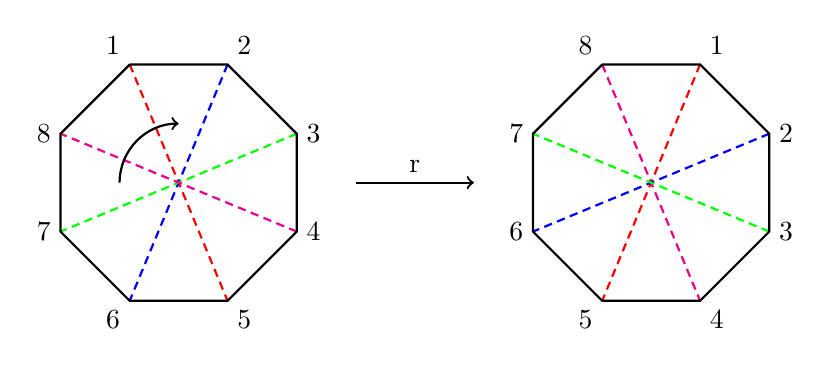
\begin{tikzpicture}[scale=1.5]
    
        \pgfmathsetmacro{\s}{sqrt(2)}

        % Specifies where the x, y coordinate of the tip of
        % the unite vectors in turn
        \tikzset{}
        
        % Scope used to shift the coordinates from the basis
        \begin{scope}[shift={(0, 0, 0)}, rotate=0]

            % Coordinates of octagon in clockwise order
            \coordinate (A1) at (1 - \s, 1);
            \coordinate (A2) at (\s - 1, 1);
            \coordinate (A3) at (1, \s - 1);
            \coordinate (A4) at (1, 1 - \s);
            \coordinate (A5) at (\s - 1, -1);
            \coordinate (A6) at (1 - \s, -1);
            \coordinate (A7) at (-1, 1 - \s);
            \coordinate (A8) at (-1, \s - 1);

            \node at (A1)[above left] {1};
            \node at (A2)[above right] {2};
            \node at (A3)[right] {3};
            \node at (A4)[right] {4};
            \node at (A5)[below right] {5};
            \node at (A6)[below left] {6};
            \node at (A7)[left] {7};
            \node at (A8)[left] {8};

        
            \coordinate (B1) at ($(A1) + (4, 0)$);
            \coordinate (B2) at ($(A2) + (4, 0)$);
            \coordinate (B3) at ($(A3) + (4, 0)$);
            \coordinate (B4) at ($(A4) + (4, 0)$);
            \coordinate (B5) at ($(A5) + (4, 0)$);
            \coordinate (B6) at ($(A6) + (4, 0)$);
            \coordinate (B7) at ($(A7) + (4, 0)$);
            \coordinate (B8) at ($(A8) + (4, 0)$);

            \node at (B1)[above left] {8};
            \node at (B2)[above right] {1};
            \node at (B3)[right] {2};
            \node at (B4)[right] {3};
            \node at (B5)[below right] {4};
            \node at (B6)[below left] {5};
            \node at (B7)[left] {6};
            \node at (B8)[left] {7};
        \end{scope}

        % Draws the coordinate system basis with unit side lengths
        % Is usually transparent, remove to see it for reference
        \begin{scope}[thick, line width=1, transparent]
            \draw (0, 0, 0) -- (1, 0, 0);
            \draw (0, 0, 0) -- (0, 1, 0);
            \draw (0, 0, 0) -- (0, 0, 1);
        \end{scope}

        \begin{scope}[thick, densely dashed]
            \draw[red] (A1) -- (A5);
            \draw[blue] (A2) -- (A6);
            \draw[green] (A3) -- (A7);
            \draw[magenta] (A4) -- (A8);

            \draw[magenta] (B1) -- (B5);
            \draw[red] (B2) -- (B6);
            \draw[blue] (B3) -- (B7);
            \draw[green] (B4) -- (B8);
        \end{scope}      

        \begin{scope}[thick]
            \draw (A1) -- (A2) -- (A3) -- (A4) -- (A5)
                -- (A6) -- (A7) -- (A8) -- (A1);

                \draw (B1) -- (B2) -- (B3) -- (B4) -- (B5)
                -- (B6) -- (B7) -- (B8) -- (B1);

                \draw[->] (1.5 , 0) -- (2.5, 0);
                \node at (2, 0)[above]{r};

                \draw[->] (-0.5, 0) arc (0:-90:-0.5);
        \end{scope}

        \end{tikzpicture}

        \caption{\label{fig:figure1} Octagon being rotated.}
    \end{figure} 


    \begin{figure}[H]
        \centering
        % figure is a tikz drawing
        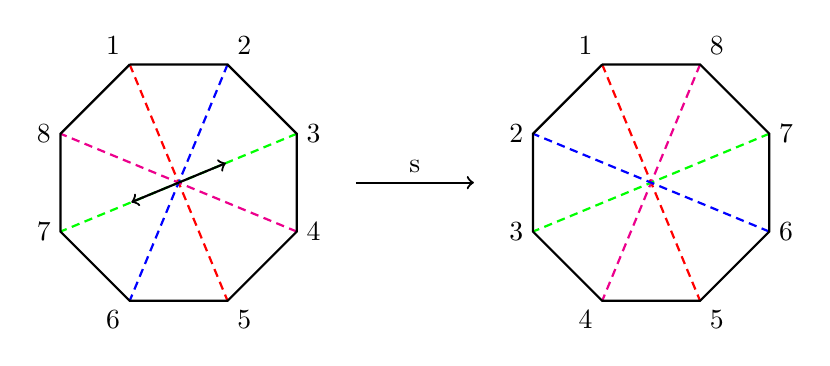
\begin{tikzpicture}[scale=1.5]

        \pgfmathsetmacro{\s}{sqrt(2)}

        % Specifies where the x, y coordinate of the tip of
        % the unite vectors in turn
        \tikzset{}
        
        % Scope used to shift the coordinates from the basis
        \begin{scope}[shift={(0, 0, 0)}, rotate=0]

            % Coordinates of octagon in clockwise order
            \coordinate (A1) at (1 - \s, 1);
            \coordinate (A2) at (\s - 1, 1);
            \coordinate (A3) at (1, \s - 1);
            \coordinate (A4) at (1, 1 - \s);
            \coordinate (A5) at (\s - 1, -1);
            \coordinate (A6) at (1 - \s, -1);
            \coordinate (A7) at (-1, 1 - \s);
            \coordinate (A8) at (-1, \s - 1);

            \node at (A1)[above left] {1};
            \node at (A2)[above right] {2};
            \node at (A3)[right] {3};
            \node at (A4)[right] {4};
            \node at (A5)[below right] {5};
            \node at (A6)[below left] {6};
            \node at (A7)[left] {7};
            \node at (A8)[left] {8};

        
            \coordinate (B1) at ($(A1) + (4, 0)$);
            \coordinate (B2) at ($(A2) + (4, 0)$);
            \coordinate (B3) at ($(A3) + (4, 0)$);
            \coordinate (B4) at ($(A4) + (4, 0)$);
            \coordinate (B5) at ($(A5) + (4, 0)$);
            \coordinate (B6) at ($(A6) + (4, 0)$);
            \coordinate (B7) at ($(A7) + (4, 0)$);
            \coordinate (B8) at ($(A8) + (4, 0)$);

            \node at (B1)[above left] {1};
            \node at (B2)[above right] {8};
            \node at (B3)[right] {7};
            \node at (B4)[right] {6};
            \node at (B5)[below right] {5};
            \node at (B6)[below left] {4};
            \node at (B7)[left] {3};
            \node at (B8)[left] {2};

            \path (A3) -- (A7) coordinate[pos=0.3](D1)
            coordinate[pos=0.7](D2);
        \end{scope}

        % Draws the coordinate system basis with unit side lengths
        % Is usually transparent, remove to see it for reference
        \begin{scope}[thick, line width=1, transparent]
            \draw (0, 0, 0) -- (1, 0, 0);
            \draw (0, 0, 0) -- (0, 1, 0);
            \draw (0, 0, 0) -- (0, 0, 1);
        \end{scope}

        \begin{scope}[thick, densely dashed]
            \draw[red] (A1) -- (A5);
            \draw[blue] (A2) -- (A6);
            \draw[green] (A3) -- (A7);
            \draw[magenta] (A4) -- (A8);

            \draw[red] (B1) -- (B5);
            \draw[magenta] (B2) -- (B6);
            \draw[green] (B3) -- (B7);
            \draw[blue] (B4) -- (B8);
        \end{scope}     
        
        \begin{scope}[thick]
            \draw (A1) -- (A2) -- (A3) -- (A4) -- (A5)
                -- (A6) -- (A7) -- (A8) -- (A1);

                \draw (B1) -- (B2) -- (B3) -- (B4) -- (B5)
                -- (B6) -- (B7) -- (B8) -- (B1);

                \draw[->] (1.5 , 0) -- (2.5, 0);
                \node at (2, 0)[above]{s};
                
            \draw[<->] (D1) -- (D2);
        \end{scope}

        \end{tikzpicture}

        \caption{\label{fig:figure1} Octagon being reflected
        around the line passing through 1 and 5.}
    \end{figure} 

    Now, every element $p_k$ in $S$ is in itself a set of opposing
    vertices $\{k, k + \sfrac{n}{2}\}$.
    To show that what we have is a group action,
    we first note that if a pair of opposite vertices $p_k$
    is mapped to $p_l$,
    then it doesn't matter how the vertices are permuted,
    so there are several ways of mapping a diagonal to another. \\
    To start, we don't have to worry that a vertex can
    be mapped to a new vertex in such a way as the set of opposite
    vertices changes
    as we've already demonstrated that can't happen.
    So we can solely focus on the way the opposite vertices are permuted.
    First, we know that $1 \cdot p_k = p_k$ for all diagonals in
    the $n$-gon,
    since 1 doesn't transform the $n$-gon in any way.
    On the other hand, for any two transformations $x, y \in D_{2n}$,
    $x \cdot y \cdot p_k =  (x \circ y) \cdot p_k$
    since composition is associative in $D_{2n}$.
    This proves that we have a group action\\
    Now, the kernel of this action is the set of elements that
    leave every pair of opposite vertices $p_k$ in place.
    The only transformation that leaves ever vertex where it is is 1.
    But as we noted before,
    we can permute the vertices so long as the diagonals remain in place.
    In other words, we need a transformation that only swaps the places
    of $k$ and $k + \sfrac{n}{2}$ for all $k$.
    The only transformation that does that,
    (which in this case, does it for all of the pairs),
    is $r^{\sfrac{n}{2}}$,
    which maps 1 to $\sfrac{n}{2}$, 2 to $\sfrac{n}{2} + 1$ \dots
    $k$ to $\sfrac{n}{2} + (k-1)$.
    There are no symmetries that fix some vertices in place
    and permute others along their diagonals.
    So the kernel of the action is the set $\{1, r^{\sfrac{n}{2}}\}$.


    \section*{Exercise 13}
    The \textit{left regular action} of a group $G$
    is the ation performed by $G$ on itself defined by
    $g \cdot h = gh$ $\forall g, h \in G$.
    The kernel of this group is the set of elements $a$
    such that $ah = h$ $\forall h \in G$.
    By definition, this property is satisfied by the identity 1,
    which is unique.
    So the kernel is the set $\{1\}$.

    
    \section*{Exercise 14}
    Proof that for a non-abelian group $G$, the action by $G$ on itself
    defined by $g \cdot h = hg$ $\forall g, h \in G$
    does not satisfy the axioms of a (left) group action: \\
    While we do have $1 \cdot g = g1 = g$,
    for $a, b, c \in G$,
    $a \cdot b \cdot c = a \cdot cb = cba = (ba) \cdot c$.
    Since the group is not abelian, not all $ab = ba$,
    so the operation is not associative,
    Meaning that it is not a (left) group action.


    \section*{Exercise 15}
    Proof that for any group $G$, the action by $G$ on itself
    defined by $g \cdot h = hg^{-1}$ $\forall g, h \in G$
    is a (left) group action: \\
    We do have $1 \cdot g = g1^{-1} = g1 = g$,
    and we also have, for $a, b, c \in G$,
    $a \cdot b \cdot c = a \cdot cb^{-1}
    = cb^{-1}a^{-1}
    = c(ab)^{-1}
    = (ab) \cdot c$.
    Since the action is associative,
    that means it is a (left) group action.


    \section*{Exercise 16}
    Proof that for any group $G$, the action by $G$ on itself
    defined by $g \cdot h = ghg^{-1}$ $\forall g, h \in G$
    is a (left) group action (called a \textit{conjugation}): \\
    We do have $1 \cdot g = 1g1^{-1} = 1g1 = g$,
    and we also have, for $a, b, c \in G$,
    $a \cdot b \cdot c = a \cdot bcb^{-1}
    = abcb^{-1}a^{-1}
    = (ab)c(ab)^{-1}
    = (ab) \cdot c$.
    Since the action is associative,
    that means it is a (left) group action.


    \section*{Exercise 17 $***$}
    Proof that for a group $G$ that acts on itself by conjugation
    (defined in exercise 1.1.7.16
    as $g \cdot h = ghg^{-1}$ $\forall g, h \in G$),
    for a fixed $g \in G$,
    the map $\phi: G \to G$ defined by $\phi(h) = ghg^{-1}$
    is an isomorphism (automorphism in this case): \\
    Since conjugation was shown to be a group action
    in exercise 1.1.7.16,
    that would make the action of a fixed $g \in G$ a permutation
    of the set $G$.
    So the map $\phi$ defined by this action must be a bijection. \\
    Moreover, $\forall h, k \in G$,
    we have $\phi(hk) = ghkg^{-1}
    = gh1kg^{-1}
    = ghg^{-1}gkg^{-1}
    = \phi(g)\phi(k)$.
    So $\phi$ is a homomorphism,
    which coupled with its being a bijection, makes it an isomorphism,
    and by extension, an automorphism. \\ 
    In exercise 1.1.6.2, we proved that for any isomorphism $\varphi$,
    $|x| = |\varphi(x)|$.
    So we can deduce that for any element $x \in G$, $|g| = |gxg^{-1}|$. \\
    Proof that for any subset $A$ of $G$,
    if $gAg^{-1} = \{gag^{-1} \mid a \in A\}$
    then $|A| = |gAg^{-1}|$: \\
    Since conjugation, the action of $g$ on $G$, is a (left) group action,
    that makes it a permutation of $G$,
    which makes it bijective, meaning it is injective
    (we could have also used the fact that $\phi$ is an isomorphism
    and by extension, a bijection).
    So each element in $A$ maps to a different element in $G$
    when the action is applied,
    so the set resulting from the group action must have the same
    cardinality as $A$, so $|A| = |gAg^{-1}|$.


    \section*{Exercise 18 $***$}
    Let $H$ be a group acting on a set $A$.
    Proof that the relation $\sim$ on $A$ defined by $a \sim b$ if and only
    if $a = hb$ for some $h \in H$ is an equivalence relation: \\
    To show that a relation is an equivalence relation,
    we need to show that it is reflective, symmetric, and transitive. \\
    If $a = hb$ implies that $a \sim b$,
    then $a = 1a$ where $1 \in H$,
    so $a \sim a$,
    so $\sim$ is reflective. \\
    Moreover,
    $a \sim b \implies a = hb \implies h^{-1}a = b \implies b \sim a$,
    so $\sim$ is symmetric. \\
    Finally, $a \sim b$ and $b \sim c$
    implies that $a = hb$ and $b = kc$ for $h, k \in H$,
    so $a = hkc = (hk)c$ where $hk \in H$,
    which means that $a \sim c$,
    so $\sim$ is transitive. \\
    This makes $\sim$ an equivalence relation.
    For each $x \in A$, the equivalence of $x$ under $\sim$ is called
    the \textit{orbit of $x$ under the action of $H$}.
    The different orbits under the action of $H$ partition $A$
    (no overlap and no elements left out).
    (Note that the orbit of $x$ and the orbit of $y$ where $y$ is
    an element of the orbit of $x$ are the same orbit, meaning any element
    in the equivalence class can serve as its representative).


    \section*{Exercise 19 $***$}
    Let $H$ be a subgroup of a finite group $G$,
    and let $H$ act on $G$ by left multiplication ($h \cdot g = hg$).
    For $x \in G$, let $\orbit$ be the orbit of $x$ under the action of $H$.
    Proof that the map $\phi: H \to \orbit$ defined by $\phi(h) = hx$
    is a bijection: \\
    Since $x$ isa fixed value,
    then for $h, k \in H$,
    if $h \neq k$,
    we have $\phi(h) = hx \neq kx = \phi(k)$.
    So $\phi$ is injective.
    Moreover, for each element $y$ in $\orbit$, $x \sim y$,
    so $y = hx$ for some $h \in H$ by definition.
    So every element in $\orbit$ is associated with an element in $h$,
    which makes $\phi$ surjective,
    making the mapping bijective.
    So $|H| = |\orbit|$ for all orbits under the action of $H$. \\
    Proof of \textit{Lagrange's Theorem} that if $H \leqslant G$,
    then $|H| \mid |G|$: \\
    We now know that $|H| = |\orbit|$ for all orbits under the action of $H$.
    Since all orbits have the same size as the subgroup $|H|$,
    all orbits must have the same cardinality.
    And from exercise 1.1.7.18,
    we know that the orbits of $G$ partition the set $G$,
    so if $|\orbit| = n$, then $|G| = nm$ for some $m \in \Z$.
    Since $|H| = |\orbit| = n$, that means that $|H| \mid |G|$.


    \section*{Exercise 20 $***$}
    Proof that the group of rigid motions of a tetrahedron in $\R^3$ $G$
    is isomorphic to a subgroup of $S_4$: \\
    Consider the set $S = \{1, 2, 3 ,4\}$ which represents the vertices of
    a tetrahedron (which has 4).
    Consider the action of the group $G$ on $S$,
    where each transformation in $G$ permutes $S$ in the same way that
    the transformation permutes the vertices of the tetrahedron.
    We know this is a group action since 1 by definition does not transform 
    the tetrahedron,
    and because composition is associative
    (same proof as exercise 1.1.7.11). \\

    % Triangle figure
    \begin{figure}[H]
        \centering
        % figure is a tikz drawing
        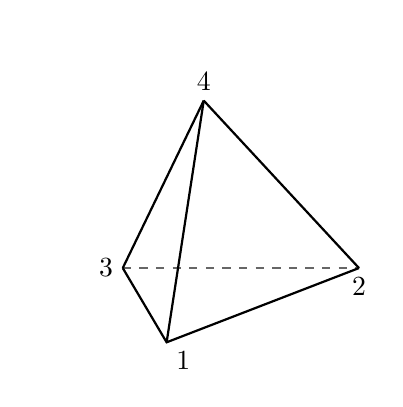
\begin{tikzpicture}[scale=3]
        % Tetrahedron formulae
        \pgfmathsetmacro{\side}{1}
        \pgfmathsetmacro{\halfside}{\side/2}
        \pgfmathsetmacro{\height}{\side * (sqrt(2/3))}
        \pgfmathsetmacro{\halfheight}{\height / 2}
        \pgfmathsetmacro{\altitude}{(\side * sqrt(3)) / 2}

        % Scope used to shift the coordinates from the basis
        \begin{scope}[shift={(0, 0, 0)}, rotate=0]
            % Triangle base
            \coordinate (A1) at (0, 0, 0);
            \coordinate (A2) at (\side, 0, 0);
            \coordinate (A3) at (\halfside, 0, \height);
            % Triangle tip
            \coordinate (B) at (\halfside, \altitude, \halfheight);

            \node at (A3) [below right] {$1$};
            \node at (A2) [below] {$2$};
            \node at (A1) [left] {$3$};
            \node at (B) [above] {$4$};

        \end{scope}

        % Draws the coordinate system basis with unit side lengths
        % Is usually transparent, remove to see it for reference
        \begin{scope}[thick, blue, line width=3, opacity=0.4, transparent]
            \draw (0, 0, 0) -- (1, 0, 0);
            \draw (0, 0, 0) -- (0, 1, 0);
            \draw (0, 0, 0) -- (0, 0, 1);   
        \end{scope}

        \begin{scope}[thick]
            \draw (A2) -- (A3) -- (A1);   
            \draw (B) -- (A1) ;
            \draw (B) -- (A2);
            \draw (B) -- (A3);
        \end{scope}

        \begin{scope}[thick,dashed,opacity=0.6]
            \draw (A1) -- (A2);
        \end{scope}

    \end{tikzpicture}

        \caption{\label{fig:figure1} Tetrahedron whose vertices
        correspond to $S = \{1, 2, 3, 4\}$.}
    \end{figure}

    Since this is a group action, then by definition,
    it corresponds to a permutation representation,
    which is a homomorphism $\phi: G \to S_4$.
    So $G$ is homomorphic to $S_4$. \\
    Now consider the subset of $S_4$, $\phi(G)$.
    From exercise 1.1.6.13, we know that the image of $G$ in $S_4$
    when $\phi$ is a homomorphism is a subgroup of $S_4$.
    So $\phi(G) \leqslant S_4$.
    Finally, we note that the map $\phi: G \to \phi(G)$
    is by definition surjective
    (since $\phi(G)$ only contains the elements of $S_4$ that are images
    of elements in $G$).
    And, $\phi$ is injective, since permutations are considered 
    distinct only if the result of their transformation permutes the
    vertices in a different way,
    meaning that each element in $G$ maps to a unique element in $S_4$.
    So $\phi: G \to \phi(G)$ is bijective and a homomorphism,
    making it an isomorphism,
    which means that $G$ is isomorphic to a subgroup of $S_4$.


    \section*{Exercise 21 $***$}
    Proof that the group of rigid motions of a cube in $\R^3$ $G$
    is isomorphic to $S_4$: \\
    Consider the set $S = \{1, 2, 3, 4\}$ which represents
    the 4 diagonals (or opposite vertices) of a tetrahedron (which has 4).
    As stated in exercise 1.1.7.12,
    since rigid motions leave the relative positions of vertices intact,
    opposite vertices remain intact after a transformation,
    meaning that we can uniquely identify the elements of the group of
    rigid motions in the way they permute the diagonals ($S$).
    So consider the action of the group $G$ on $S$,
    where each transformation in $G$ permutes $S$ in the same way that
    the transformation permutes the diagonals of the cube.
    We know this is a group action since 1 by definition does not transform 
    the cube,
    and because composition is associative
    (same proof as exercise 1.1.7.11). \\

    % Square figure
    \begin{figure}[H]
    \centering
    % figure is a tikz drawing
        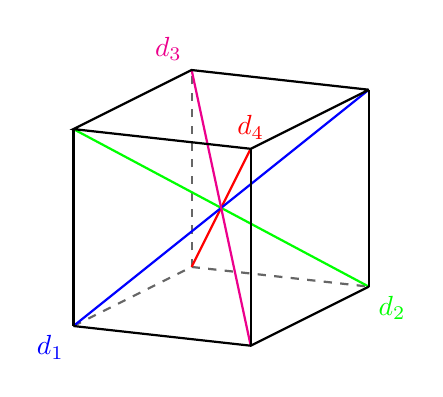
\begin{tikzpicture}[scale=2.5]
        % Cube formulae
        \pgfmathsetmacro{\side}{1}
        \pgfmathsetmacro{\halfside}{\side/2}
        \pgfmathsetmacro{\extra}{0.5}

        % Specifies where the x, y coordinate of the tip of
        % the unite vectors in turn
        \tikzset{
            x={(0.9cm, -0.1cm)}, y={(0cm,1cm)}, z={(-0.6cm,-0.3cm)},
        }

        % Scope used to shift the coordinates from the basis
        \begin{scope}[shift={(0, 0, 0)}, rotate=0]
            % Lower square
            \coordinate (A1) at (0, 0, 0);
            \coordinate (A2) at (\side, 0, 0);
            \coordinate (A3) at (\side, 0, \side);
            \coordinate (A4) at (0, 0, \side);
            % Upper square
            \coordinate (B1) at (0, \side, 0);
            \coordinate (B2) at (\side, \side, 0);
            \coordinate (B3) at (\side, \side, \side);
            \coordinate (B4) at (0, \side, \side);

            \node at (A2) [below right, green] {$d_2$};
            \node at (A4) [below left, blue] {$d_1$};
            \node at (B1) [above left, magenta] {$d_3$};
            \node at (B3) [above, red] {$d_4$};


        \end{scope}

        % Draws the coordinate system basis with unit side lengths
        % Is usually transparent, remove to see it for reference
        \begin{scope}[thick, blue, line width=3, opacity=0.4, transparent]
            \draw (0, 0, 0) -- (1, 0, 0);
            \draw (0, 0, 0) -- (0, 1, 0);
            \draw (0, 0, 0) -- (0, 0, 1);   
        \end{scope}

        \begin{scope}[thick,dashed,opacity=0.6]
            \draw (A1) -- (A2);
            \draw (A1) -- (B1);
            \draw (A4) -- (A1);
        \end{scope}

        \begin{scope}[thick]
            \draw[red] (A1) -- (B3);
            \draw[green] (A2) -- (B4);
            \draw[blue] (A4) -- (B2);
            \draw[magenta] (A3) -- (B1);

            \draw (A2) -- (A3) -- (A4);   
            \draw (B2) -- (A2);
            \draw (B3) -- (A3);
            \draw (B4) -- (A4);
            \draw (B2) -- (B3) -- (B4) -- (B1) -- (B2);   
        \end{scope}

        \end{tikzpicture}

        \caption{\label{fig:figure1} Cube whose diagonals correspond
        to $S = \{1, 2, 3, 4\}$.}
    \end{figure}

    Since this is a group action, then by definition,
    it corresponds to a permutation representation,
    which is a homomorphism $\phi: G \to S_4$.
    So $G$ is homomorphic to $S_4$. \\
    We know that $\phi$ is injective, since permutations are considered 
    distinct only if the result of their transformation places the
    diagonals to different places (if all of the diagonals are mapped
    the same way, then the two transformations are equivalent),
    meaning that each element in $G$ maps to a unique element in $S_4$.
    We also know from exercise 1.1.2.10 that there are 24 rigid
    motions that can be perofrmed on a cube while keeping its shape intact,
    so $|G| = 24 = 4! = |S_4|$.
    So that makes $\phi$ bijective, which makes the homomorphism
    an isomorphism.
    Hence, $G \cong S_4$.

    
    \section*{Exercise 22 $***$}
    Proof that the group of rigid motions of an octahedron in $\R^3$ $G$
    is isomorphic to a subgroup of $S_4$: \\
    Consider the set $S = \{1, 2, 3 ,4\}$ which represents the opposite
    faces of the octahedron (which has 4 pairs).
    As stated in exercise 1.1.7.12,
    since rigid motions leave the relative positions of vertices intact,
    opposite faces remain intact after a transformation,
    meaning that we can uniquely identify the elements of the group of
    rigid motions in the way they permute the pairs of faces ($S$).
    Consider the action of the group $G$ on $S$,
    where each transformation in $G$ permutes $S$ in the same way that
    the transformation permutes the pairs of faces of the tetrahedron.
    We know this is a group action since 1 by definition does not transform 
    the tetrahedron,
    and because composition is associative
    (same proof as exercise 1.1.7.11). \\

     % Octahedron figure
    \begin{figure}[H]
        \centering
        % figure is a tikz drawing
        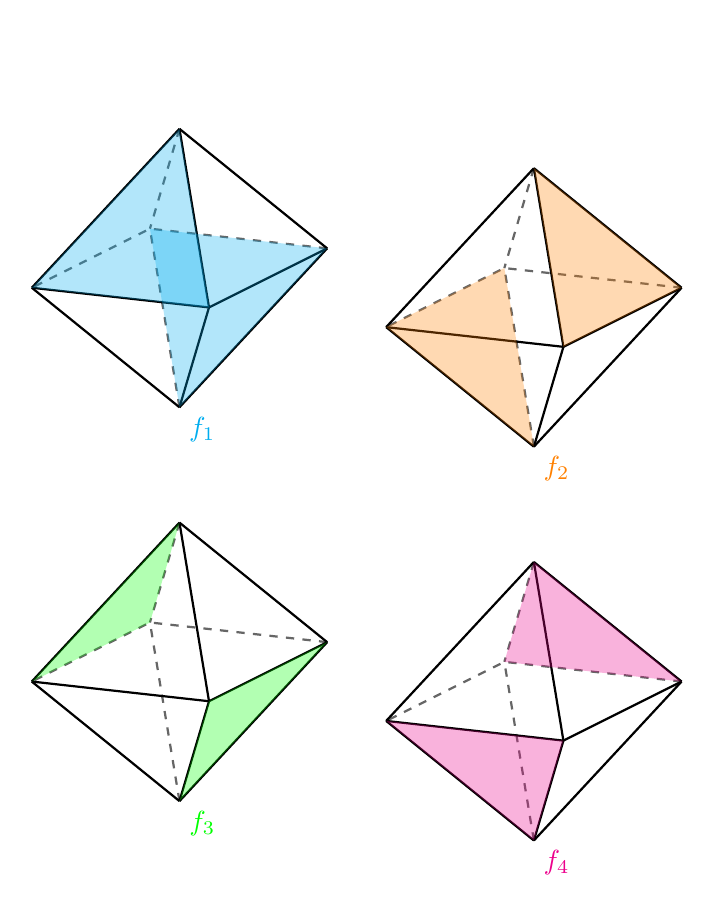
\begin{tikzpicture}[scale=2.5]
        % Octahedron formulae
        \pgfmathsetmacro{\side}{1}
        \pgfmathsetmacro{\halfside}{\side/2}
        \pgfmathsetmacro{\altitude}{\side/sqrt(2)}

        % Specifies where the x, y coordinate of the tip of
        % the unite vectors in turn
        \tikzset{
            x={(0.9cm, -0.1cm)}, y={(0cm,1cm)}, z={(-0.6cm,-0.3cm)},
        }
        
        % Scope used to shift the coordinates from the basis
        \begin{scope}[shift={(0, 0, 0)}, rotate=0]
            % Base square
            \coordinate (A1) at (0, 0, 0);
            \coordinate (A2) at (\side, 0, 0);
            \coordinate (A3) at (\side, 0, \side);
            \coordinate (A4) at (0, 0, \side);
            % Upper and lower tips
            \coordinate (B1) at (\halfside, \altitude, \halfside);
            \coordinate (B2) at (\halfside, -\altitude, \halfside);

            \coordinate (C1) at ($(A1) + (2, 0, 0)$);
            \coordinate (C2) at ($(A2) + (2, 0, 0)$);
            \coordinate (C3) at ($(A3) + (2, 0, 0)$);
            \coordinate (C4) at ($(A4) + (2, 0, 0)$);
            \coordinate (D1) at ($(B1) + (2, 0, 0)$);
            \coordinate (D2) at ($(B2) + (2, 0, 0)$);

            \coordinate (E1) at ($(A1) + (0, -2, 0)$);
            \coordinate (E2) at ($(A2) + (0, -2, 0)$);
            \coordinate (E3) at ($(A3) + (0, -2, 0)$);
            \coordinate (E4) at ($(A4) + (0, -2, 0)$);
            \coordinate (F1) at ($(B1) + (0, -2, 0)$);
            \coordinate (F2) at ($(B2) + (0, -2, 0)$);

            \coordinate (G1) at ($(A1) + (2, -2, 0)$);
            \coordinate (G2) at ($(A2) + (2, -2, 0)$);
            \coordinate (G3) at ($(A3) + (2, -2, 0)$);
            \coordinate (G4) at ($(A4) + (2, -2, 0)$);
            \coordinate (H1) at ($(B1) + (2, -2, 0)$);
            \coordinate (H2) at ($(B2) + (2, -2, 0)$);

            \node at (B2) [below right, cyan] {$f_1$};
            \node at (D2) [below right, orange] {$f_2$};
            \node at (F2) [below right, green] {$f_3$};
            \node at (H2) [below right, magenta] {$f_4$};
        \end{scope}



        % Draws the coordinate system basis with unit side lengths
        % Is usually transparent, remove to see it for reference
        \begin{scope}[thick, blue, line width=3, opacity=0.4, transparent]
            \draw (0, 0, 0) -- (1, 0, 0);
            \draw (0, 0, 0) -- (0, 1, 0);
            \draw (0, 0, 0) -- (0, 0, 1);   
        \end{scope}

        \begin{scope}[thick]
            \draw (A2) -- (A3) -- (A4);  
            \draw (B1) -- (A2);
            \draw (B1) -- (A3);
            \draw (B2) -- (A3);
            \draw (B2) -- (A4);
            \draw (B1) -- (A4);
            \draw (B2) -- (A2); 

            \draw (C2) -- (C3) -- (C4);  
            \draw (D1) -- (C2);
            \draw (D1) -- (C3);
            \draw (D2) -- (C3);
            \draw (D2) -- (C4);
            \draw (D1) -- (C4);
            \draw (D2) -- (C2); 

            \draw (E2) -- (E3) -- (E4);  
            \draw (F1) -- (E2);
            \draw (F1) -- (E3);
            \draw (F2) -- (E3);
            \draw (F2) -- (E4);
            \draw (F1) -- (E4);
            \draw (F2) -- (E2); 

            \draw (G2) -- (G3) -- (G4);  
            \draw (H1) -- (G2);
            \draw (H1) -- (G3);
            \draw (H2) -- (G3);
            \draw (H2) -- (G4);
            \draw (H1) -- (G4);
            \draw (H2) -- (G2); 
        \end{scope}

        \begin{scope}[thick,dashed,opacity=0.6]
            \draw (B2) -- (A1);    
            \draw (B1) -- (A1); 
            \draw (A2) -- (A1) -- (A4);  

            \draw (D2) -- (C1);    
            \draw (D1) -- (C1); 
            \draw (C2) -- (C1) -- (C4);  

            \draw (F2) -- (E1);    
            \draw (F1) -- (E1); 
            \draw (E2) -- (E1) -- (E4);
            
            \draw (H2) -- (G1);    
            \draw (H1) -- (G1); 
            \draw (G2) -- (G1) -- (G4);  
        \end{scope}

        \begin{scope}[thick,dashed,opacity=0.3]
            \fill[cyan] (A3) -- (A4) -- (B1);
            \fill[cyan] (A2) -- (A1) -- (B2);

            \fill[orange] (C2) -- (C3) -- (D1);
            \fill[orange] (C4) -- (C1) -- (D2);

            \fill[green] (E4) -- (E1) -- (F1);
            \fill[green] (E2) -- (E3) -- (F2);

            \fill[magenta] (G1) -- (G2) -- (H1);
            \fill[magenta] (G3) -- (G4) -- (H2);
        \end{scope}

        \end{tikzpicture}

        \caption{\label{fig:figure1} Octahedron whose pairs of faces
        correspond to $S = \{ 1, 2, 3, 4 \}$.}
    \end{figure}
    
    Since this is a group action, then by definition,
    it corresponds to a permutation representation,
    which is a homomorphism $\phi: G \to S_4$.
    So $G$ is homomorphic to $S_4$. \\
    Now consider the subset of $S_4$, $\phi(G)$.
    From exercise 1.1.6.13, we know that the image of $G$ in $S_4$
    when $\phi$ is a homomorphism is a subgroup of $S_4$.
    So $\phi(G) \leqslant S_4$.
    Finally, we note that the map $\phi: G \to \phi(G)$
    is by definition surjective
    (since $\phi(G)$ only contains the elements of $S_4$ that are images
    of elements in $G$).
    And, $\phi$ is injective, since permutations are considered 
    distinct only if the result of their transformation places each
    face in a different place (if all of them are mapped to the same
    pairs, then the two transofrmations are equivalent),
    meaning that each element in $G$ maps to a unique element in $S_4$.
    So $\phi: G \to \phi(G)$ is bijective and a homomorphism,
    making it an isomorphism,
    which means that $G$ is isomorphic to a subgroup of $S_4$. \\
    However, note that since $\phi: G \to S_4$ is injective for the same
    reason that $\phi: G \to \phi(G)$ is,
    then by exercise 1.1.2.10, $|G| = 24 = 4! = |S_4|$,
    so $\phi: G \to S_4$ is bijective, making it an isomorphism.
    That means that the subgroup of $S_4$ to which $G$ is isomorphic
    is $S_4$ itself (all groups are as subgroup of themselves). \\
    As we know from exercise 1.1.7.21,
    the group $G'$ of rigid motions of a cube in $\R^3$
    is also isomorphic to $S_4$.
    Since isomorphy is an equivalence relation, it is transitive.
    So as $G \cong S_4$ and $S_4 \cong G'$, we have $G \cong G'$.

    
    \section*{Exercise 23 $***$}
    Consider the action of the group of rigid motions of a cube in $\R^3$
    $G$ on the set $S = \{1, 2, 3\}$,
    where each transformation in $G$ permutes $S$ in the same way that
    the transformation permutes the pairs of faces of the cube.
    Proof that the action is not faithful: \\
    As stated in exercise 1.1.7.12,
    since rigid motions leave the relative positions of vertices intact,
    opposite faces remain opposite after a transformation.
    However, unlike the other group actions in exercises, 1.1.7.20, 1.1.7.21,
    and 1.1.2.22, we can't uniquely identify the transformations of $G$
    in the way $G$ permutes the pairs of opposite faces
    because the action is not faithful. \\
    First, for the action of the group $G$ on $S$,
    where each transformation in $G$ permutes $S$ in the same way that
    it permutes the pairs of oppposite faces,
    we can show that this is indeed a group action
    as 1 by definition does not transform the cube,
    and because composition is associative
    (same proof as exercise 1.1.7.11). \\
    Now to show that it is not faithful,
    we need to find two transformations that map the pairs of opposite faces
    faces similarly while being two distinct transformations.
    This is possible because there are several ways of mapping a
    pair of faces to another.
    For instance, two different mappings of vertices can correspond to
    the same pair of faces ending up in a specific position,
    as there is no restriction on which face is mapped to which other
    face in the pairs.
    Another way of saying that different transformations correspond to the
    same permutation of faces is to say the permutation representation
    homomorphism of this action $\phi: G \to S_3$ is not injective.
    We know that $\phi$ is well defined because it is a homomorphism
    (a result of the fact that opposite faces remain opposite after a 
    transformation).
    However, we have $|G| = 24$ (as shown in exercise 1.1.2.10),
    and we have $|S_3| = 3! = 6$. 
    Since the mapping is well defined, every element in $G$ must map
    to one element in $S_3$,
    but as $S_3$ has a smaller order than $G$,
    then by the pigeonnhole principle, 
    some elements in $G$ will map to the same element in $S_3$,
    meaning that $\phi$ is not injective,
    so the action is not faithful. \\

    % Square figure
    \begin{figure}[H]
    \centering
    % figure is a tikz drawing
        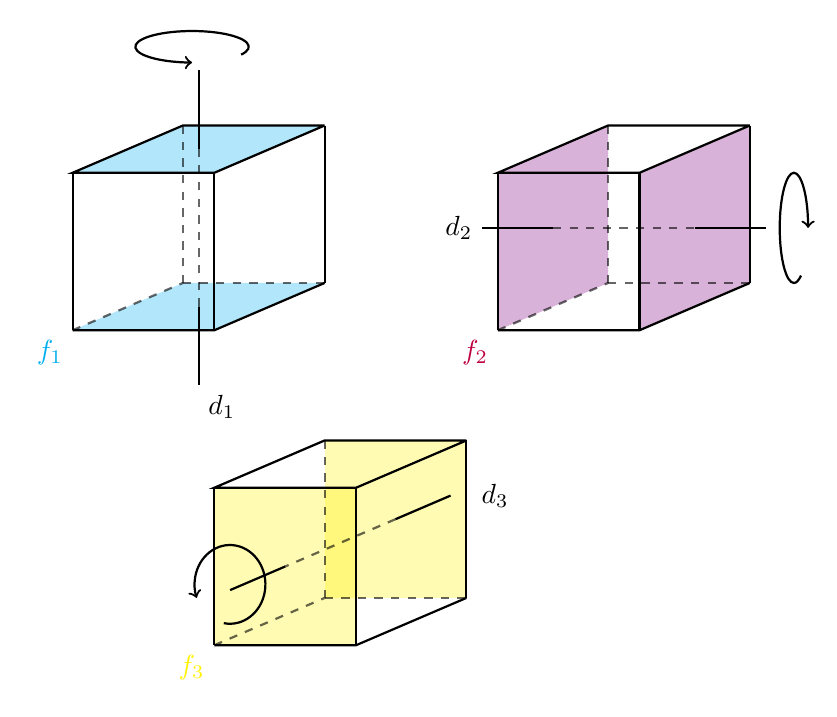
\begin{tikzpicture}[scale=2]
        % Cube formulae
        \pgfmathsetmacro{\side}{1}
        \pgfmathsetmacro{\extra}{0.5}

        \tikzset{
            x={(0.9cm, 0)}, y={(0cm,1cm)}, z={(-0.7cm,-0.3cm)},
        }

        % Scope used to shift the coordinates from the basis
        \begin{scope}[shift={(0, 0, 0)}, rotate=0]
            \coordinate (A1) at (0, 0, 0);
            \coordinate (A2) at (\side, 0, 0);
            \coordinate (A3) at (\side, 0, \side);
            \coordinate (A4) at (0, 0, \side);
            \coordinate (B1) at (0, \side, 0);
            \coordinate (B2) at (\side, \side, 0);
            \coordinate (B3) at (\side, \side, \side);
            \coordinate (B4) at (0, \side, \side);

            \coordinate (CEN1) at ($0.25*(A1) + 0.25*(A2) + 0.25*(A3)
            + 0.25*(A4)$);
            \coordinate (CEN2) at ($(CEN1) + (0, \side, 0)$);
            \path (CEN1) -- (CEN2) coordinate[pos=-0.5](O1)
            coordinate[pos=1.5](O2);

            \coordinate (C1) at ($(A1) + (3, 0, 0)$);
            \coordinate (C2) at ($(A2) + (3, 0, 0)$);
            \coordinate (C3) at ($(A3) + (3, 0, 0)$);
            \coordinate (C4) at ($(A4) + (3, 0, 0)$);
            \coordinate (D1) at ($(B1) + (3, 0, 0)$);
            \coordinate (D2) at ($(B2) + (3, 0, 0)$);
            \coordinate (D3) at ($(B3) + (3, 0, 0)$);
            \coordinate (D4) at ($(B4) + (3, 0, 0)$);

            \coordinate (CEN3) at ($0.25*(C1) + 0.25*(D1) + 0.25*(C4)
            + 0.25*(D4)$);
            \coordinate (CEN4) at ($(CEN3) + (\side, 0, 0)$);
            \path (CEN4) -- (CEN3) coordinate[pos=-0.5](O3)
            coordinate[pos=1.5](O4);

            \coordinate (E1) at ($(A1) + (1, -2, 0)$);
            \coordinate (E2) at ($(A2) + (1, -2, 0)$);
            \coordinate (E3) at ($(A3) + (1, -2, 0)$);
            \coordinate (E4) at ($(A4) + (1, -2, 0)$);
            \coordinate (F1) at ($(B1) + (1, -2, 0)$);
            \coordinate (F2) at ($(B2) + (1, -2, 0)$);
            \coordinate (F3) at ($(B3) + (1, -2, 0)$);
            \coordinate (F4) at ($(B4) + (1, -2, 0)$);

            \coordinate (CEN5) at ($0.25*(E1) + 0.25*(E2) + 0.25*(F2)
            + 0.25*(F1)$);
            \coordinate (CEN6) at ($(CEN5) + (0, 0, \side)$);
            \path (CEN5) -- (CEN6) coordinate[pos=-0.5](O5)
            coordinate[pos=1.5](O6);

            \node at (A4) [below left, cyan] {$f_1$};
            \node at (C4) [below left, purple] {$f_2$};
            \node at (E4) [below left, yellow] {$f_3$};

            \node at (O1) [below right] {$d_1$};
            \node at (O4) [left] {$d_2$};
            \node at ($(O5) + (0.15, 0, 0)$) [right] {$d_3$};

        \end{scope}

        % Draws the coordinate system basis with unit side lengths
        % Is usually transparent, remove to see it for reference
        \begin{scope}[thick, blue, line width=3, opacity=0.4, transparent]
            \draw (0, 0, 0) -- (1, 0, 0);
            \draw (0, 0, 0) -- (0, 1, 0);
            \draw (0, 0, 0) -- (0, 0, 1);   
        \end{scope}

        \begin{scope}[thick,dashed,opacity=0.3]
            \fill[cyan] (A1) -- (A2) -- (A3) -- (A4);
            \fill[cyan] (B1) -- (B2) -- (B3) -- (B4);

            \fill[violet] (C1) -- (C4) -- (D4) -- (D1);
            \fill[violet] (C2) -- (D2) -- (D3) -- (C3);

            \fill[yellow] (E1) -- (E2) -- (F2) -- (F1);
            \fill[yellow] (E4) -- (F4) -- (F3) -- (E3);
        \end{scope}

        \begin{scope}[thick,dashed,opacity=0.6]
            \draw (A1) -- (A2);
            \draw (A1) -- (B1);
            \draw (A4) -- (A1);

            \draw (C1) -- (C2);
            \draw (C1) -- (D1);
            \draw (C4) -- (C1);

            \draw (E1) -- (E2);
            \draw (E1) -- (F1);
            \draw (E4) -- (E1);

            \draw (CEN1) -- (CEN2);
            \draw (CEN3) -- (CEN4);            
            \draw (CEN5) -- (CEN6);
        \end{scope}

        \begin{scope}[thick]
            \draw (A2) -- (A3) -- (A4);   
            \draw (B2) -- (A2);
            \draw (B3) -- (A3);
            \draw (B4) -- (A4);
            \draw (B2) -- (B3) -- (B4) -- (B1) -- (B2);   

            \draw (C2) -- (C3) -- (C4);   
            \draw (D2) -- (C2);
            \draw (D3) -- (C3);
            \draw (D4) -- (C4);
            \draw (D2) -- (D3) -- (D4) -- (D1) -- (D2);   

            \draw (E2) -- (E3) -- (E4);   
            \draw (F2) -- (E2);
            \draw (F3) -- (E3);
            \draw (F4) -- (E4);
            \draw (F2) -- (F3) -- (F4) -- (F1) -- (F2);  
            
            \draw (CEN1) -- (O1);
            \draw (CEN3) -- (O4);            
            \draw (CEN5) -- (O5);
            \draw (CEN2) -- (O2);
            \draw (CEN4) -- (O3);            
            \draw (CEN6) -- (O6);

            \draw[->] ($(O2) + (0.3, 0.1, 0)$) arc [start angle=-30,
            end angle=270, x radius=0.4, y radius=0.1];

            \draw[<-] ($(O3) + (0.3, 0, 0)$) arc [start angle=0,
            end angle=300, x radius=0.1, y radius=0.35];

            \draw[->] ($(O6) + (0.5, 0, 0.7)$) arc [start angle=-100,
            end angle=200, x radius=0.25, y radius=0.25];
        \end{scope}

        \end{tikzpicture}

        \caption{\label{fig:figure1} Cube whose pairs of faces correspond to
        $S = \{1, 2, 3\}$.}
    \end{figure}

    Since the action is not faithful,
    then the kernel of the action must contain more elements
    than just the identity,
    as proven in exercise 1.1.7.6.
    So the kernel is the set of rigid motion in $\R^3$ that leaves the
    pairs of faces in place,
    but does allow us to swap between the faces so long as they belong
    to the same pair.
    No transformations allow us to swap the faces of 1 pair or all 3 pairs,
    so we instead look at the transformations that swap the faces of 2
    of the pairs and leave the third pair as is: \\
    We can rotate the cube $180 \degree$ around $d_1$,
    a line that passes through the centers of the first pair of opposite
    faces. This rotation swaps the faces of the second and third pair
    of faces, but leaves the first intact. \\
    We can also rotate the cube $180 \degree$ around $d_2$,
    a line that passes through the centers of the second pair of opposite
    faces. This rotation swaps the faces of the first and third pair
    of faces, but leaves the second intact.
    And finally, we can rotate the cube $180 \degree$ around $d_3$,
    a line that passes through the centers of the third pair of opposite
    faces. This rotation swaps the faces of the first and second pair
    of faces, but leaves the third intact. \\
    So the kernel is made of the identity and these three rotations.



\end{document}
